\begin{landscape}
{
\begin{table}[htb]\centering
{\tiny{}
  \begin{tabular}{lllll}
  Container Price & Year & Source & Measured Units & Note\\\hline
               & 1965,1970,1975,1979 & Issues of Our Ocean Shipping &dollars per 100 tons-mile&Liner sector, three main cargo\\
               & 1973-1976 & Current status of marine transportation &converted dollars per TEU&Revenue and quantity on only Transpacific and Asia-Europe routes\\
               &1976-1994 & Global Container Markets Drewry Shipping Consultants &dollars by FEU &Missing 1976-1989 in Asia-Europe\\
               &1994-2009 & Review of Maritime Transport &dollars by TEU&All market-level info is available\\
              & & & &\\
  Liner price & & & &\\\hline
               &1965-2009 & Review of Maritime Transport &index rate based on 1995(=100)&Global liner freight rate\\
               & & & &\\
  Quantity & & & &\\\hline
                    &1966-1972 & Containerization International 1973&TEU& Aggregate carrying capacity for each route\\
                    &1970,1974,1978,1980 &The Container Crisis 1982 &1 million ton&
                    Aggregate quantity for each route\\
                    &1975,1978,1981,1984,1987,1990&Container transportation cost and profitability 1980/2000 &1000TEU&Aggregate quantity for each route\\
                    &1985-1997&World Sea Trade Service &1000TEU&All market-level info is available\\
                    &1994-2009 & Review of Maritime Transport &1000TEU& All market-level info is available\\
                     & & & &\\
                    &(1970,1975,1977,1978,1979) &*Issues of Our Ocean Shipping &D/W tons&Aggregate quantity for each route\\
                    &(1973)& *Containerization International 1975 &1000TEU&Aggregate quantity for each route\\
                    &(1978,1981)&*The Container market to 1990 &TEU&Aggregate carrying capacity for each route and container type\\
                    &(1983)&*World Container Data 1985 &1000TEU&Aggregate quantity for each route
  \end{tabular}
  \begin{tablenotes}
\item[a]\textit{Note:} The data sources with ($*$) are used for reference to check the consistency of the trend.
\end{tablenotes}
  }
  \caption{Overview of data sources.}
  \label{tb:overview_of_datasources}
\end{table}
\begin{figure}[!ht]
\begin{minipage}[b]{0.45\linewidth}
  \centering
  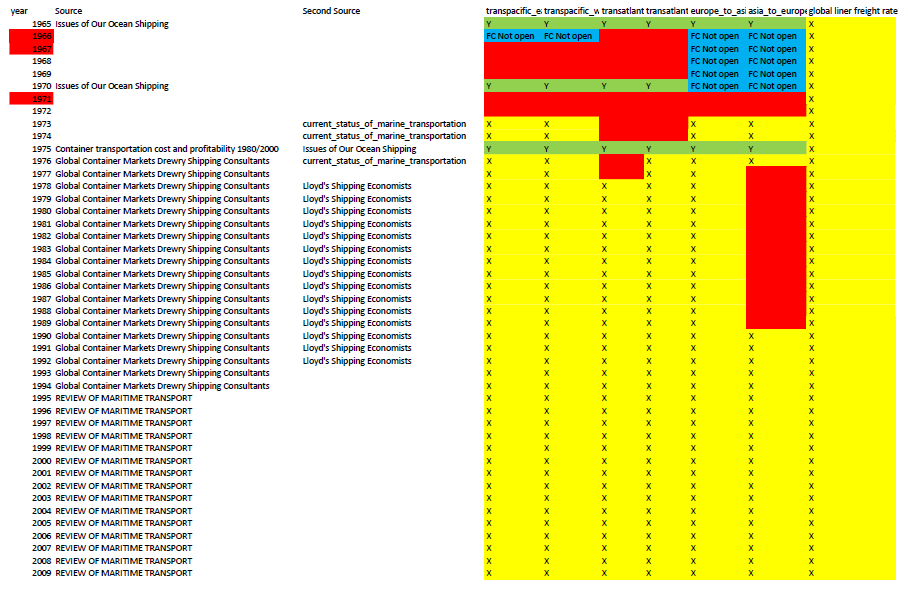
\includegraphics[height = 0.4\textheight]{freight_rate_filled_and_imputed_summary.png}
  \end{minipage}
  \begin{minipage}[b]{0.45\linewidth}
  \centering
  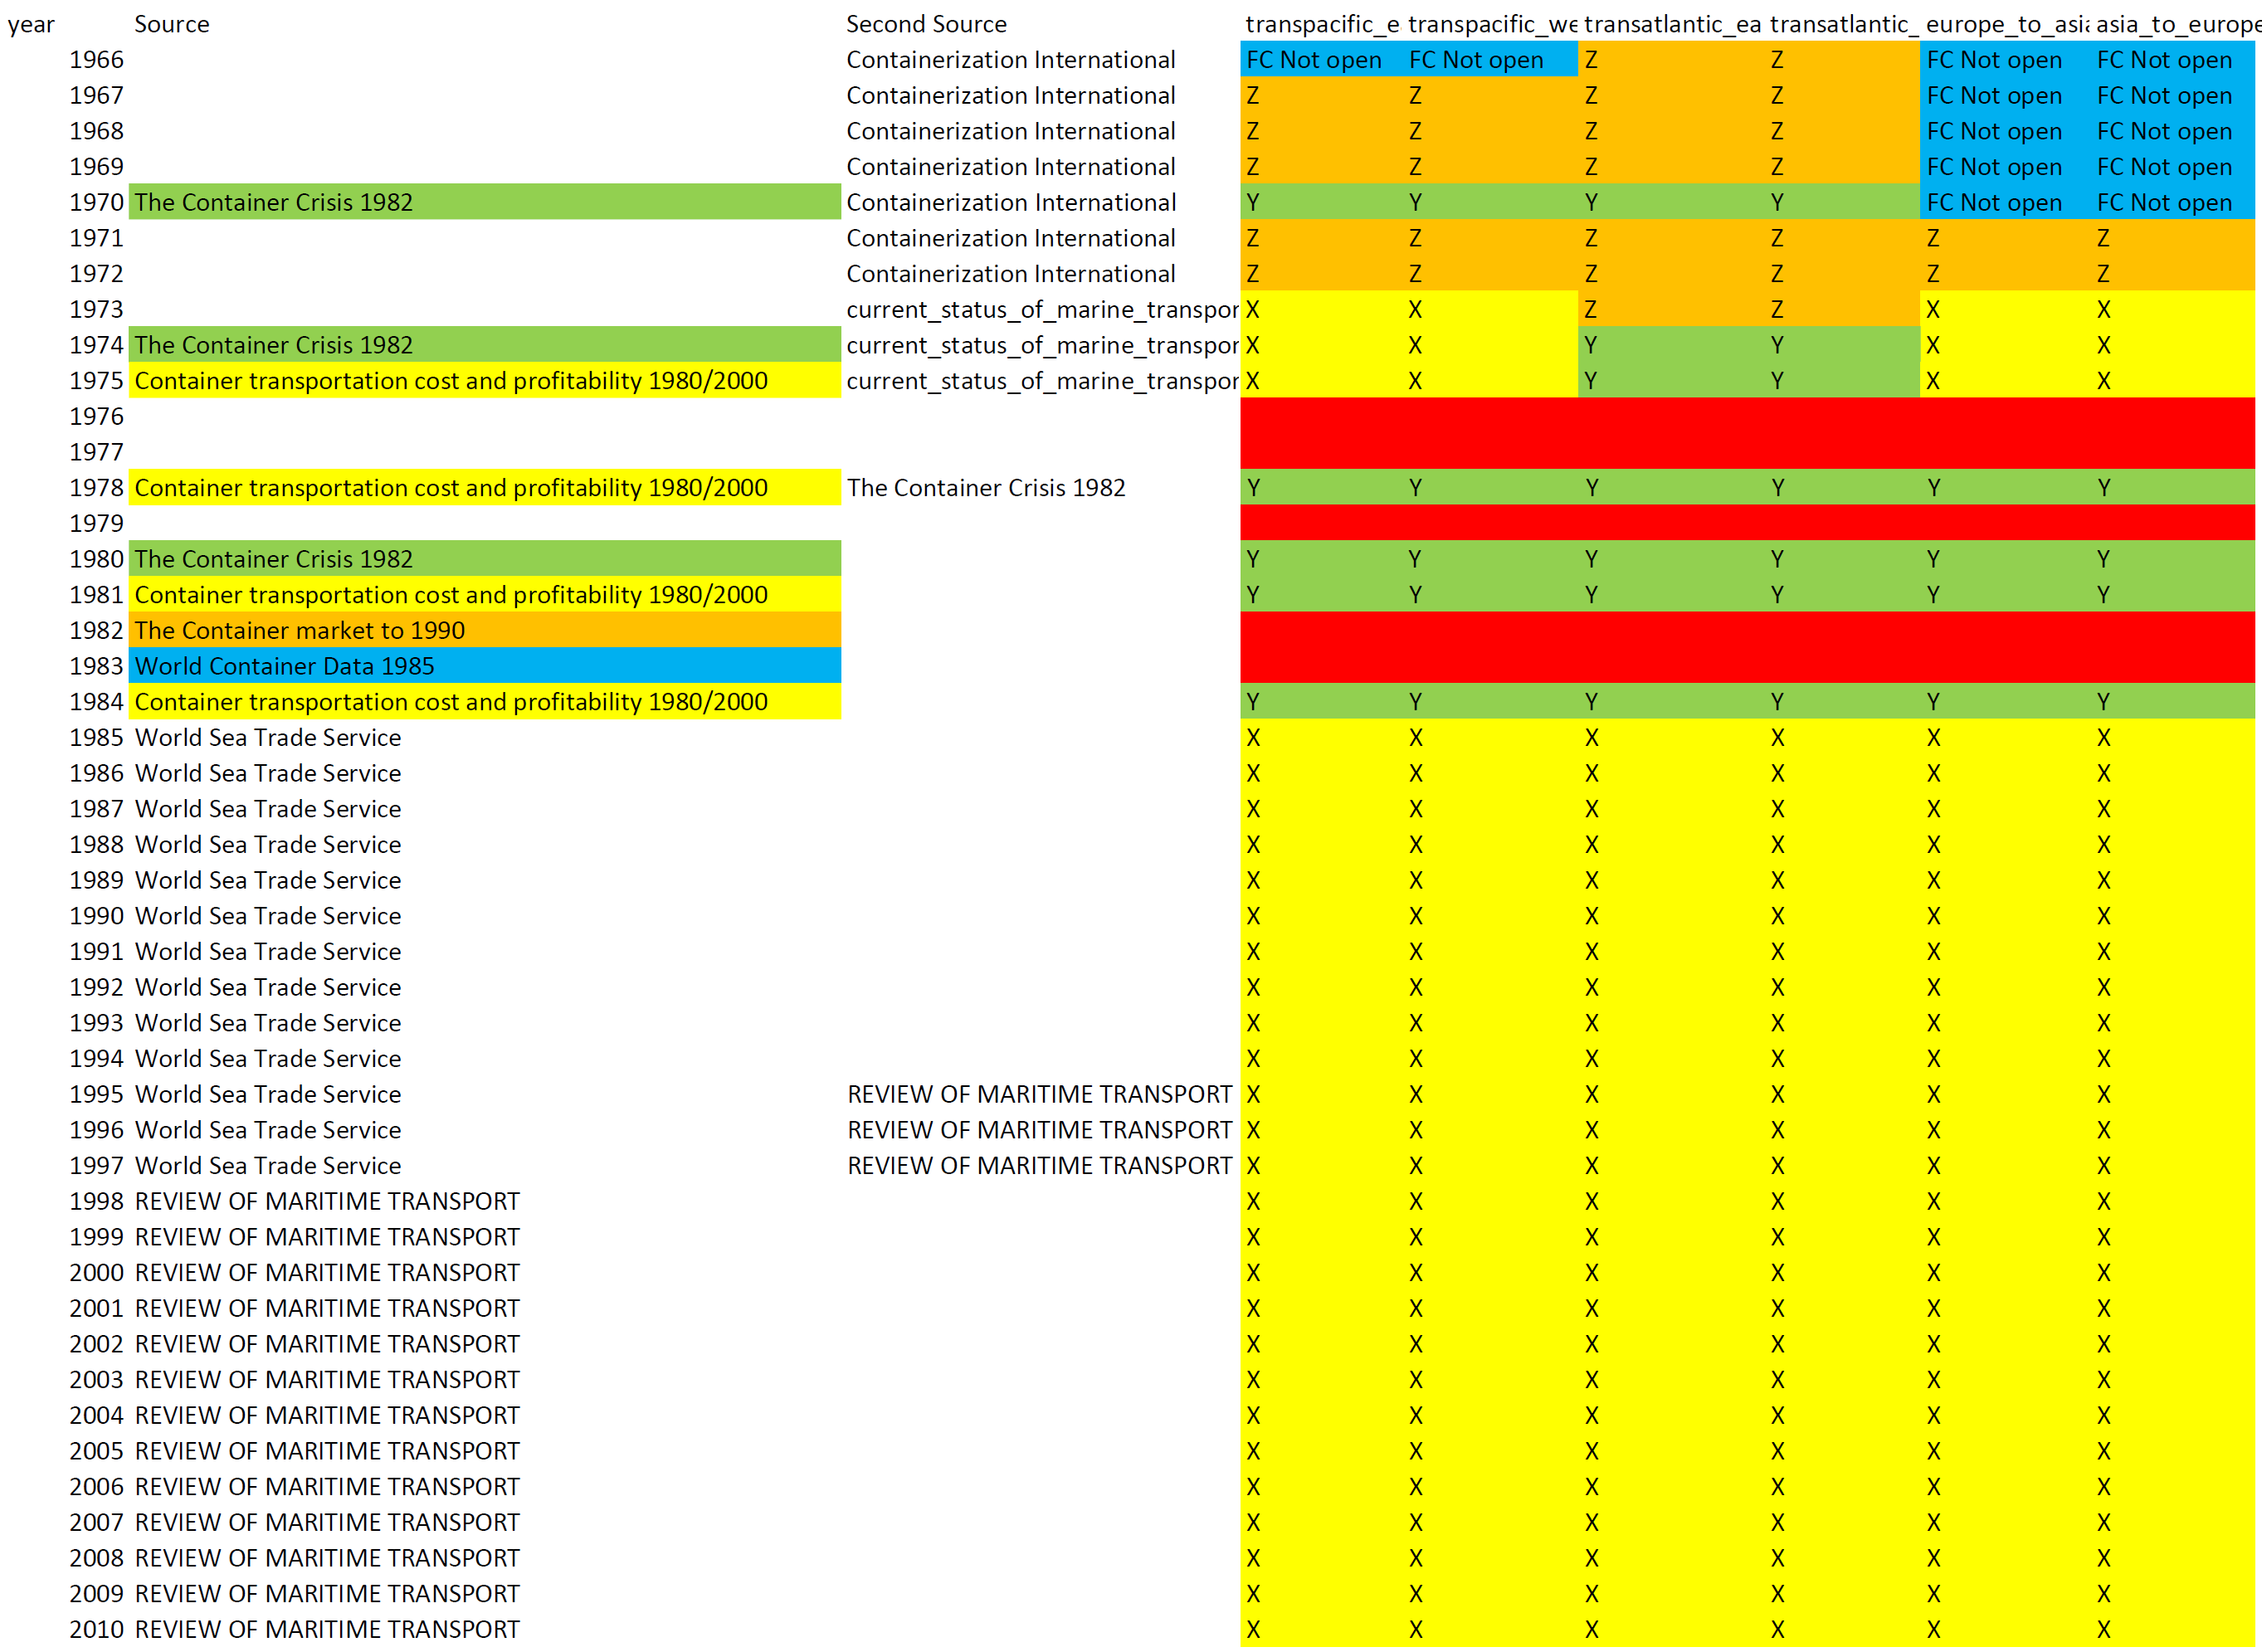
\includegraphics[height = 0.4\textheight]{traffic_amount_filled_and_imputed_summary.png}
  \end{minipage}
\caption{The observed and imputed variable cells for market-level data.}
{\tiny{}
\begin{tablenotes}
\item[a]\textit{Note:} In the yellow X cells, the route-level variables are recorded in data. In the green Y cells, the route-level cells that cannot identify the eastbound and westbound routes are recorded, so that we assign the the values based on the fixed ratio of the eastbound to the westbound in the closest period. In the orange Z cells, although route-level variables are not recorded, ship-level variables with targeted routes are available, so that we convert firm-level information into route-level variables based on the fixed ratio in the closest period. The red cells are missing values. Thus, we impute the values via interpolation based on the observed points in each route and global liner freight rate.
\end{tablenotes}
}
\end{figure}
}
\end{landscape}

\section{Data construction (Not for publication)}\label{sec:data_construction}

The container shipping industry is a fascinating laboratory for investigating industry dynamics. Because the industry started global shipping in 1966, we can find the initial state of the market dynamic structure. There is also substantial firm entry and exit in the industry, which makes the container shipping industry ideal for studying industry dynamics in global markets. Finally, the markets see the dynamics of shipping alliance, mergers, and consolidations. 

Despite the significance, a panel dataset regarding the container freight rate and shipping quantity on the three major trade routes (front-haul and back-haul separately) between 1966 and 2009 has not been available. \footnote{Similar to related papers focusing on the container freight rate panel data, \cite{luo2009econometric} use shipping demand and freight rate data between 1980 and 2007. As shipping demand, they used the world container throughput reported in the Drewry Annual Container Market Review and Forecast. The container freight rate, which is calculated as the weighted average of Transpacific, Europe-Far East and Transatlantic trades from the same data source. Because of the data limitation, they calculated the missing period (1980–1993) from the General Freight Index in the Shipping Statistics Yearbook 2007, using a simple statistical equation between container freight rate and the general freight index from 1994 to 2008.}  This note provides unified instruction and guidance to construct the dataset based on published books and publicly available data sources as much as possible, although the construction and merging processes will involve conversion and imputation errors from multiple datasets. The data sources are presented in Table \ref{tb:overview_of_datasources}. Instead of manually constructing the freight index from the commodity-level freight rate via formal but complicated processes, we adopted the tractable imputation approach, that is, linking multiple data sources that overlap information for a few years. The corresponding code is also provided to ensure that an interested researcher can replicate the construction. 

Collecting data on the container freight rate and shipping quantity, particularly before 1994, is not trivial because there is no single data source. In the subsequent subsections, we have provided detailed data construction for each container freight rate and shipping quantity.

\subsection{Container freight rate}

To construct the data regarding the container freight rate, we refer to the three data sources presented in Table  \ref{tb:overview_of_datasources} and the liner freight rate before global containerization.

\subsubsection{Shipping alliance and Liner freight rate}\label{subsec:shipping_alliance}

The liner shipping industry has traditionally formed shipping alliances like explicit cartels. Until 1984, shipping alliances played an important role in the container-shipping market. For example, in February 1967, a container shipping firm, Matson, started an operation on the Atlantic route under the freight rate contracted with one of the alliance groups, the TPFC. Thus, the container freight rate was determined by liner shipping alliances.

This unique feature allows us to use the liner freight rate to approximate the container freight rate. Figure \ref{fg:liner_freight_rate} compares the liner freight rate with the container freight rate recorded since 1995. This suggests that the container freight rate and its fluctuations can be inferred from the liner freight rate. In particular, “Issues of Our Ocean Shipping” recorded that in 1978, 76.0\%  of U.S. liner transports, 66.4\% of European liner transports, and 68.8\% of Asian and Australian liner transports were containerized. That is, more than two-thirds of the liner freight rate was determined by the container freight rate in the 1970s, as in the 1990s.


\begin{figure}[!ht]
\begin{center}
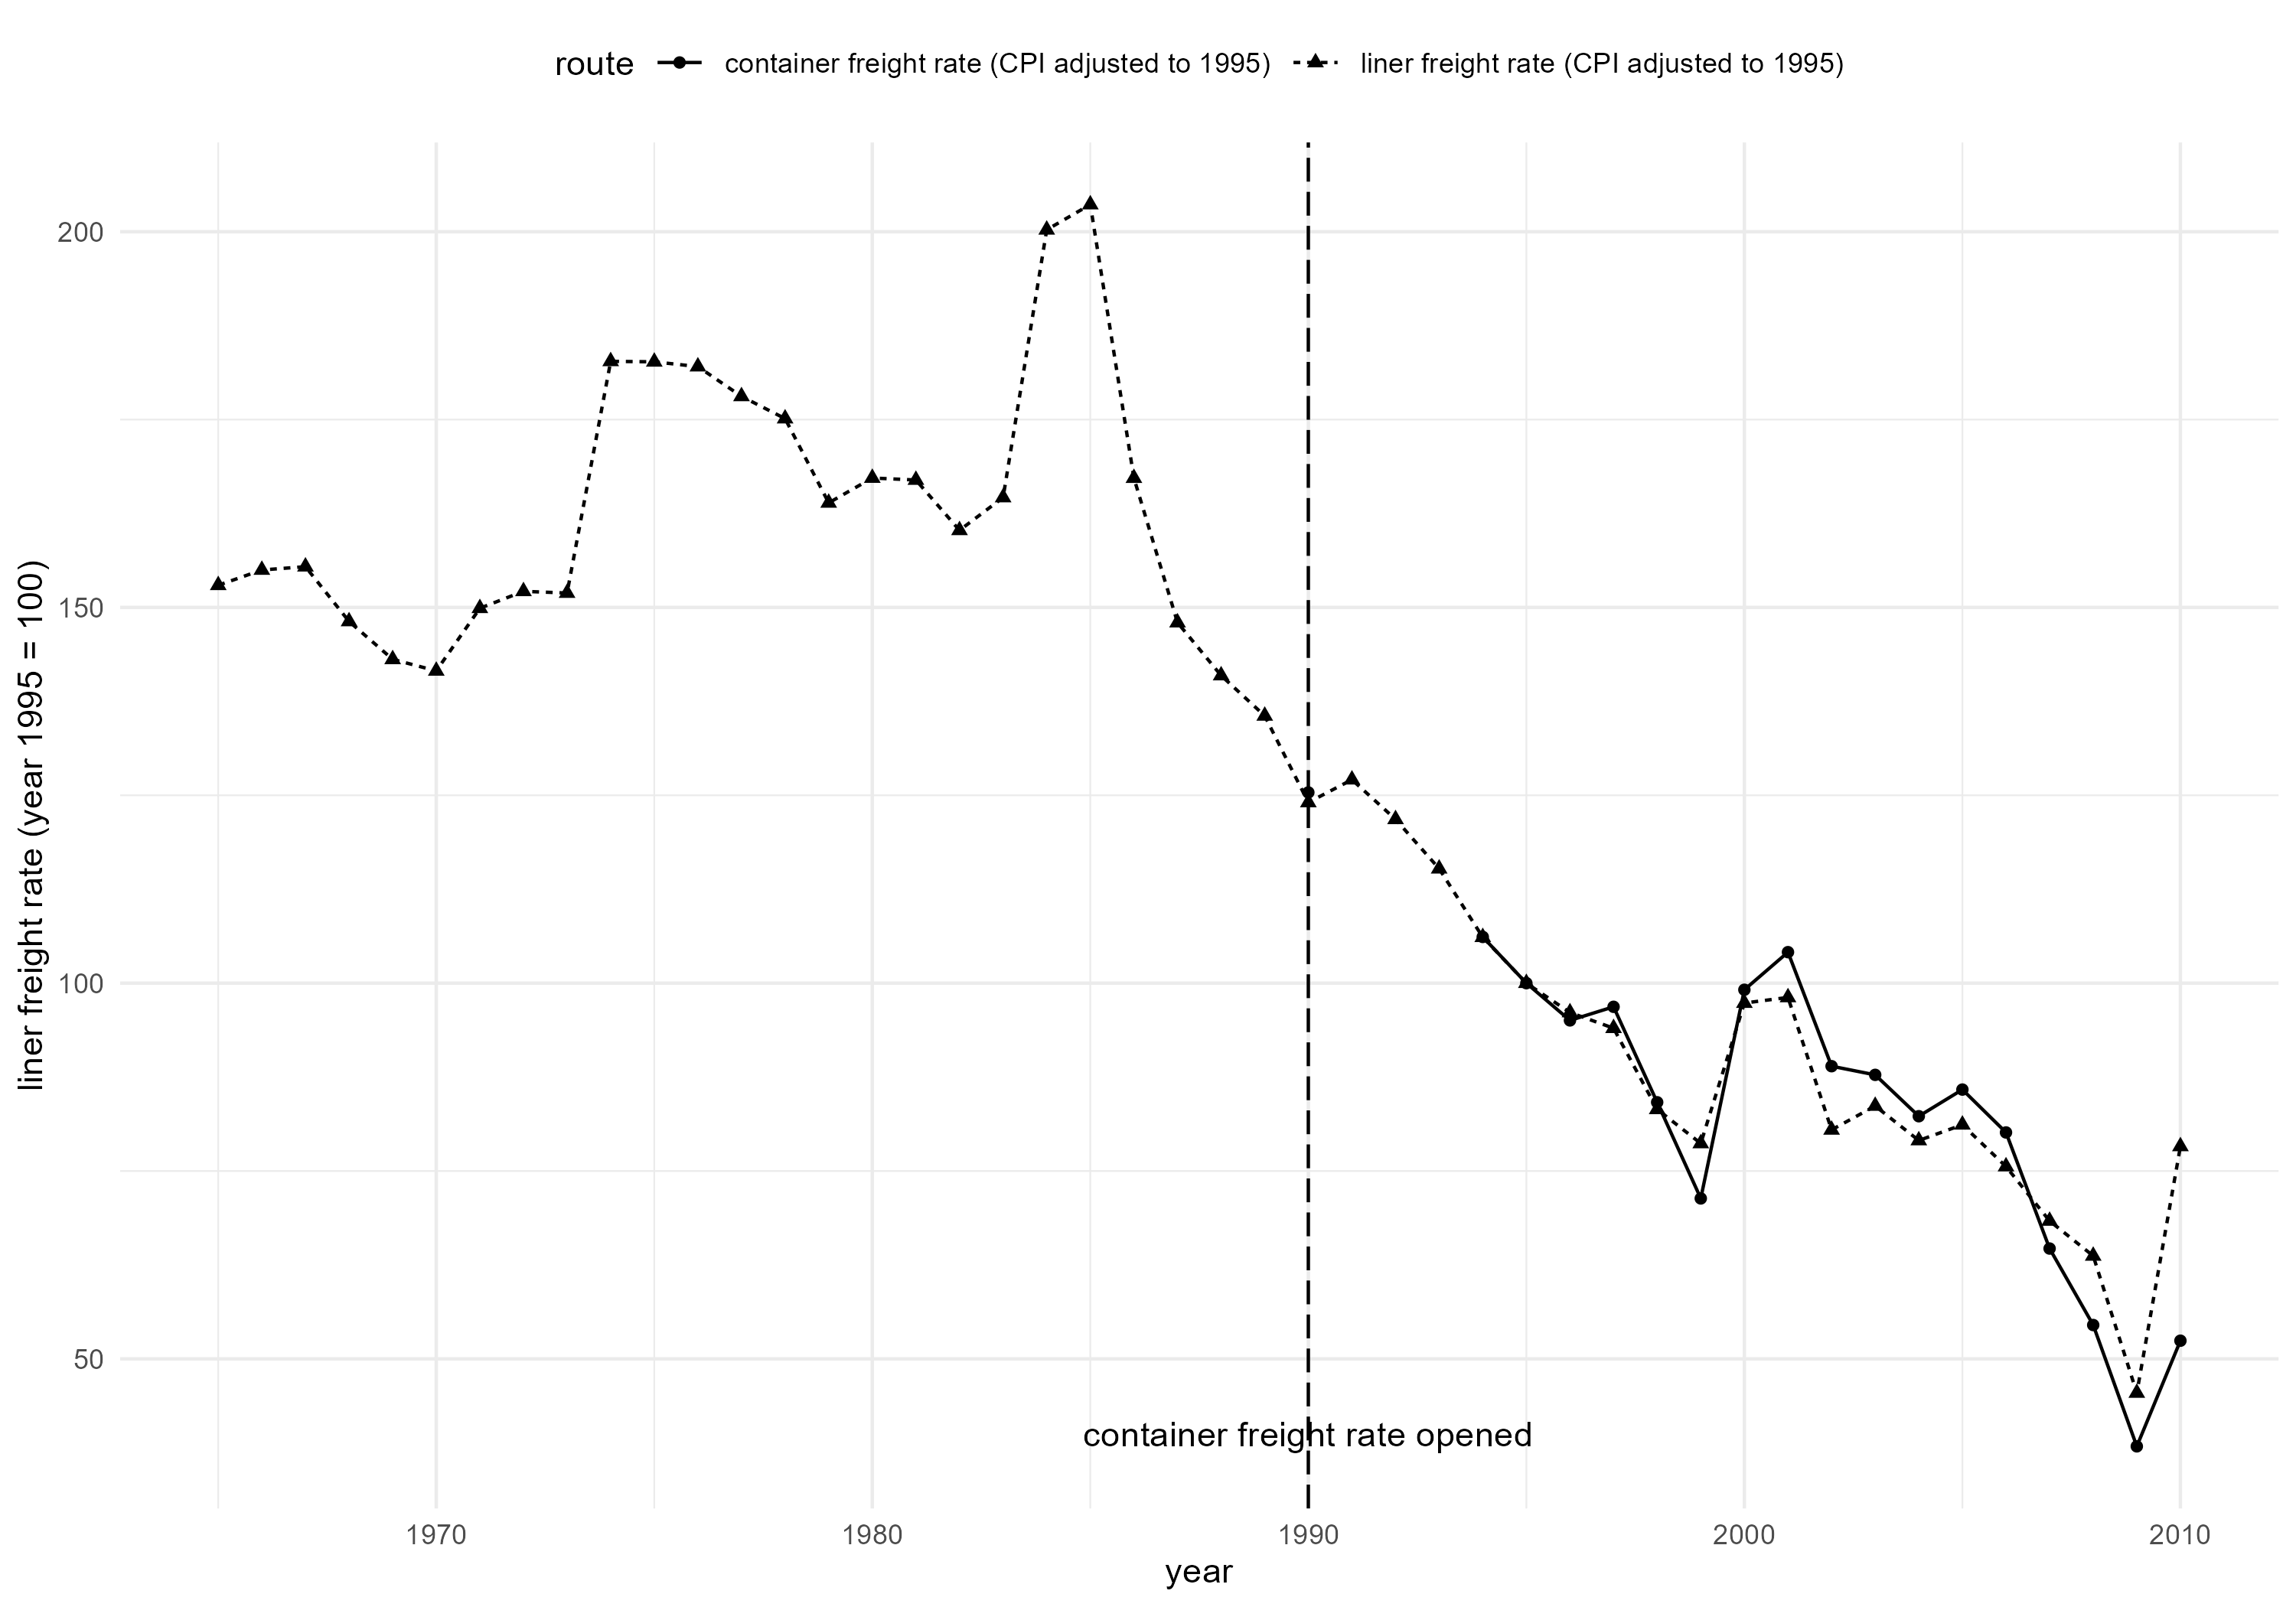
\includegraphics[height = 0.4\textheight]{figuretable/liner_freight_rate.png}
\end{center}
\caption{The trend of the liner freight rate.}
\begin{tablenotes}
\item[a]\textit{Note:} Source: \textit{Review of Maritime Transport}, published annually by UNCTAD. The measure of the price index is not explicitly mentioned in the Review of Maritime Transport.
\end{tablenotes}
\label{fg:liner_freight_rate}
\end{figure}


\subsubsection{Container freight rate between 1966 and 1975}



Data on the freight rate between 1966 (i.e., the beginning of the industry) and 1975 are missing from a single data source. Thus, we need to infer and impute data from multiple data sources and information in subsequent years. Fortunately, we can use the institutional knowledge in Section  \ref{subsec:shipping_alliance}, the liner freight rate, and the published data that overlap the data in some subsequent years in multiple data sources.

``Issues of Our Ocean Shipping" (\textit{``Wagakuni no Gaikou Kaiun Ni Tsuite", in Japanese}) records the freight rate of liner shipping on the three major routes in 1965, 1970, 1975, and 1979. The freight rates for the three types of cargo (i.e., electric appliances, clothes, and ceramic products) are available. These freight rates were measured in dollars for 100 tons per mile. The shipping miles between specific ports are listed.\footnote{For the Transpacific and Asia-Europe routes, the shipping miles between specific ports, that is, Japan-Hamburg and Japan-San Francisco routes are mentioned. However, only for the transatlantic route, the specific ports were not mentioned. Thus, we take the average of the shipping miles for Hamburg-San Francisco (i.e., west coast) and Hamburg-Halifax routes (i.e., east coast).} Using this information, we can recover the route-level container freight rates for 1965, 1970, and 1975. Finally, we assumed that the proportions of the liner and container freight rates for each route were fixed before 1975. Under this assumption, we recovered and interpolated the eastbound and westbound container freights for each route based on the fixed proportion of the liner and container freight rate and that of subsequent years, which overlaps container freight rates in multiple data sources. \footnote{The overlapped information in 1979 is a key year for merging multiple data before and after 1975. However, the freight rate swung irregularly and non-proportionally in both data sources. For making the smooth transition of the freight rate in the merged dataset, we calculated the conversion rate based on the freight rate of 1975 from \textit{Issues of our ocean shipping} and that of 1976 from \textit{Global container markets year}.}



\subsubsection{Container freight rate between 1976 and 1994}

The container industry faced significant market changes during this period. Specifically, in 1984, the maritime cartel was applied to the United States’ antitrust law to ensure the determinants of the liner freight rate changed. After 1984, it approached a competitive global market.

The data on the freight rate between 1976 and 1994 were recorded in \textit{Global Container Markets Drewry Shipping Consultants}. The recording of the freight rate starts from 1976 for the transatlantic and Transpacific routes and from 1990 for the Europe-Asia route. Thus, data on the freight rate of the Europe-Asia route between 1976 and 1989 are missing.\footnote{\textit{Global Container Markets Drewry Shipping Consultants} stated that, ``the Europe-Far East trade is the least well documented of the axial routes (page 109)".} 

For the imputation of the missing data, we assumed that the proportion of liner and container freight rates for eastbound and westbound Asia-Europe routes are fixed between 1976 and 1990. This assumption implies that there is no time-varying difference between the eastbound and westbound Asia-Europe routes. Under this assumption, we recovered the container freight rates of the eastbound and westbound Asia-Europe routes.



\subsubsection{Container freight rate after 1995}\label{subsec:freight_rate_after_1995}

The freight rate data are recorded in the  \textit{Review of Maritime Transport} which refers to \textit{Containerization International Yearbook}. The recording of freight rates began in June 1994.\footnote{\cite{jeon2022learning} stated: ``The first dataset on firm-level investment and capital is therefore supplemented with the historical price and quantity data compiled from the Review of Maritime Transport published by the United Nations that goes back to 1997." (p. 9). However, we confirm that the data in 1994 are available in \textit{Containerization International Yearbook}.} \textit{Containerization International Yearbook} mentioned that \textit{``the information is derived mainly from confidential reports provided by some of the main carriers and other public sources."} Owing to the consistency of data sources and public availability, the \textit{Review of Maritime Transport} is often used. For example, \cite{jeon2022learning} used quarterly freight data.


Processing the above steps generate the time-series data of the container freight rate for each route between 1966 and 2009. Figure \ref{fg:container_freight_rate_each_route} reveals the trend of the container freight rate, CPI-adjusted to 1995, with the liner freight rate depicted in Figure \ref{fg:liner_freight_rate}. In particular, the recovered and imputed data points in the 1960s and the 1970s quantitatively captured anecdotal and institutional evidence. First, for the transatlantic and Transpacific routes, the peak in 1976 and a sharp declining trend in 1979 were captured. Second, the container freight rate on each route corresponds to  the fluctuation of the liner freight rate.

\begin{figure}[!ht]
\begin{center}
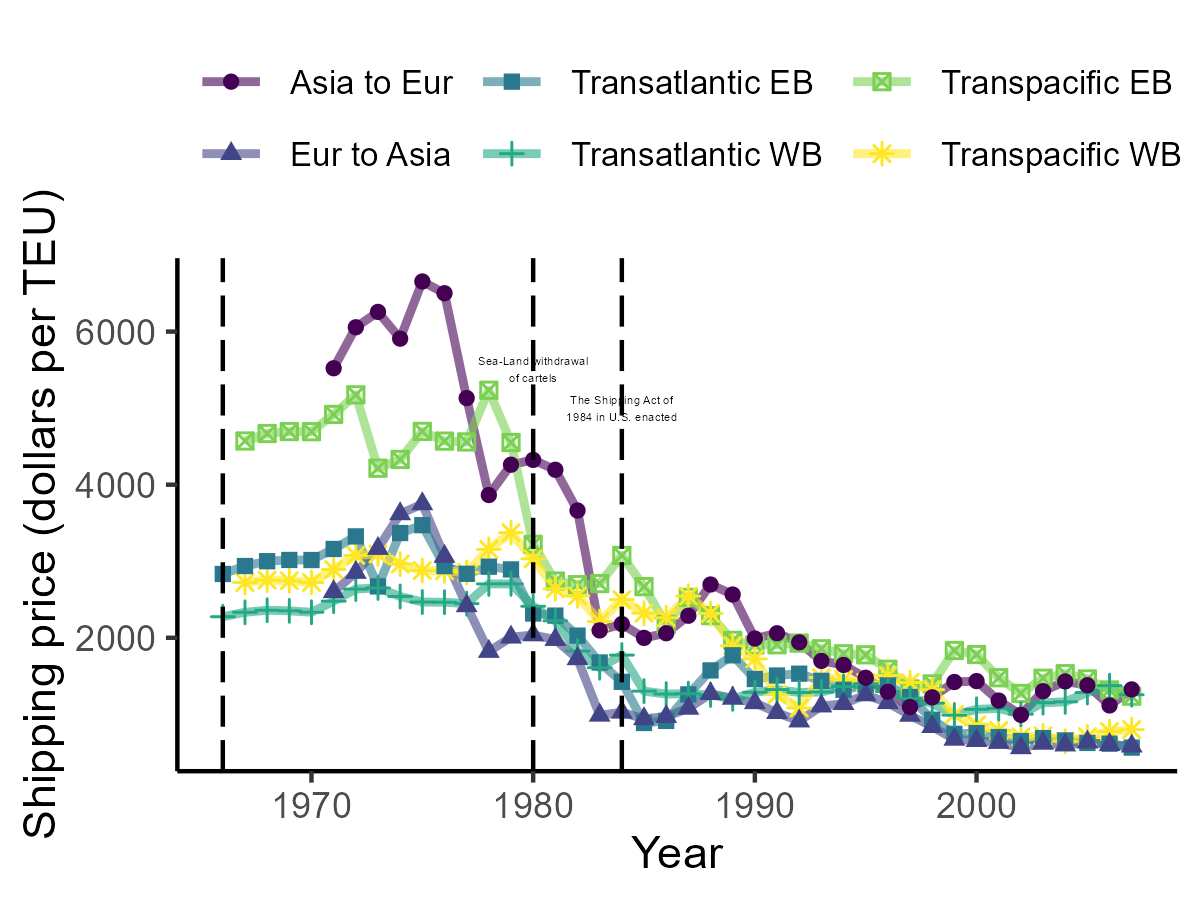
\includegraphics[height = 0.5\textheight]{figuretable/container_freight_rate_each_route.png}
\end{center}
\caption{The trend of the container freight rate.}
\label{fg:container_freight_rate_each_route}
\end{figure}

\subsection{Shipping quantity}

To construct data regarding the container trade volume, we refer to five data sources shown in Table \ref{tb:overview_of_datasources}.

\subsubsection{Shipping quantity between 1966 and 1975}

Official data on shipping quantities between 1966 and 1969 were not available. However, we could keep track of the development of container vessels during this period. First, data regarding vessel capacity were recorded in \textit{Containerization International 1973}.\footnote{``Theory and Practice of Container Shipping" (\textit{``Container Yusou no Riron to Jissai", in Japanese}). This contains the information about the launch of container ships owned by the United States main four firms, Moore-McCormack, U.S. Lines, SeaLand, and CML (American Export Isbrandtsen). This help me to identify the exact launch year only of full-container ships by the largest players, that is, United States container shipping companies. We use the data source only to check institutional evidence.} This information identifies the carrier composition on the Transatlantic, Transpacific, and Asia-Europe routes between 1966 and 1972.

Second, \textit{Review of Maritime Transport} (1971) summarizes the relationship between the annual global container carrying capacity and container capacity in 1969 and 1970 on the transatlantic route. We assume that container capacities were fully exploited during this period. This assumption is not restrictive, because the demand for container shipping was considerably high during this period. Under this assumption, the shipping quantity is recovered by calculating the total shipping quantity from the container capacity and invariant conversion rate.

% \begin{table}[ht!]
% {\tiny{}
%     \centering
%     \begin{tabular}{ccllll}
%       Year &page& Event & Firm (Group) & annual global capacity (TEU) & container capacity (TEU) \\\hline
%       Transatlantic route && &  & &\\
%       1966, Feb && 6 semi-containers& by Moore-McCormack & &\\
%       1966, Mar & p.27& 4 semi-containers& by U.S. Lines & &\\
%       1966, Apr &p.29& 4 full-containers& by SeaLand & & 0.5 million tons\\
%       1966, Sep &p.29& 4 full-containers& by CML (American Export Isbrandtsen) & & 0.4 million tons\\
%       &&&&&\\
%       1967, Sep &p.194& 3 Ro-Ro ships &by ACL & &0.75 million tons\\
%       &&&&&\\
%       1968, Feb &p.194 & 5 full-containers &by U.S. Lines & &0.65 million tons\\
%       1968, Sep &p.194 & 6 full-containers &by Sealand & &3 million tons\\
%       1968,??? &p.74 & 5 full-containers &by U.S. Lines & &?\\
%       1968,summer &p.76 & 3 full-containers &by CML (American Export Isbrandtsen) & &?\\
%       &&&&&\\
%       1969 &RMT(1971)& XX & & 66100 &714000\\
%       1970 &RMT(1971)&   & & 104700 &114200\\
%       &&&&&\\\hline
%       Tranpacific route && &  & &\\
%       1967, Sep && 7 ships &by Matson & &\\
%       && &  & &\\
%       1968, Sep && ? containers &by Japanese groups & &\\
%       && &  & &\\\hline
%       Asia-Europe route && &  & &\\
%       1970  && 1 full-container &by Nippon Yusen &&\\
%     \end{tabular}
%     \caption{The container industry historical background before 1970. Source: Review of Maritime Transport 1971.}
%     \label{tb:container_industry_history_before_1970}
% }
% \end{table}


Third, the data on shipping quantity in 1970 and 1974 were recorded in \textit{The Container Crisis 1982}, and the data for 1973 were recorded in \text{containerization international 1975}, fortunately. However, data for 1971 and 1972 were missing. The data also contains the regional levels of container shipping, that is, container traffic in Asia, North America, and Europe. One of the alternatives is the imputation approach, which employs external data that provide information about missing data.\footnote{\cite{jeon2022learning} stated that: “We set the start date for firms’’ information as the second quarter of 1966, which is the date of the first international container voyage. Then, we employed quarterly data on the value of trade by origin-destination pair from the IMF Direction of Trade Statistics database to impute the missing data on demand states from 1966: Q2-1996: Q4.” (p. 25), and “To translate the value of trade to the quantity of container trade, the demand state for the 1997–-2014 period was regressed on the de-trended value of trade. Then, the demand states for periods with missing data are constructed as predicted values from the regression. For the 1997–-2014 period, actual demand states are used.” (footnote 37).} We assign the recorded trade volume to each route in proportion based on the subsequent years.\footnote{Alternatively, we could assign the aggregate container shipping quantity to westbound and eastbound routes based on the data on the value of trade by origin-destination pair from \textit{the IMF Direction of Trade Statistics database}. We did not take the full-imputation approach because the value of trade includes goods transported by the bulk shipping service.} For missing years, we interpolate the trade volume using observed data points.



\subsubsection{Shipping quantity between 1976 and 1994}

The data on shipping quantity between 1976 and 1994 were recorded in \textit{World Sea Trade Service}, \textit{Container transportation cost and profitability 1980/2000}, \textit{The Container Crisis 1982}, and \textit{World Container Data 1985}. In particular, \textit{World Sea Trade Service} started recording data from 1985, whereas the other data sources recorded the data before 1985 but irregularly. Specifically, the quantity data for 1971, 1972, 1973, 1976, 1977, and 1979 were missing for all routes, and the quantity data for 1970, 1974, 1980, 1982, and 1983 are recorded in the total shipping quantity, summing up eastbound and westbound for each market.




\subsubsection{Shipping quantity after 1995}
The data about shipping quantity after 1995 are recorded in the  \textit{Review of Maritime Transport} and \textit{World's sea trades}. The former refers to \textit{World Sea Trade Service Review, various issues, 1996}, \textit{Journal of Commerce, various issues, 1996}, and \textit{Containerization International, various issues, 1996.} As in Section \ref{subsec:freight_rate_after_1995}, shipping quantity data are easily constructed from a single data source, that is, the  \textit{Review of Maritime Transport}. Before merging the data before and after 1995, we confirm that the discrepancy between the two data sources is small for almost all market-year observations. However, only the quantities in the transatlantic eastbound and westbound routes in 1995 were somewhat different.

Processing the above steps generate the time-series data of container shipping quantity measured by 1,000 TEU for each route between 1966 and 2009. Figure \ref{fg:container_shipping_quantity_each_route} illustrates the trend in container shipping quantity. The shipping quantity on all routes increased monotonically between 1973 and 2000. After 2000, this trend increased exponentially, particularly in the Transpacific eastbound and Europe-to-Asia routes.

\begin{figure}[!ht]
\begin{center}
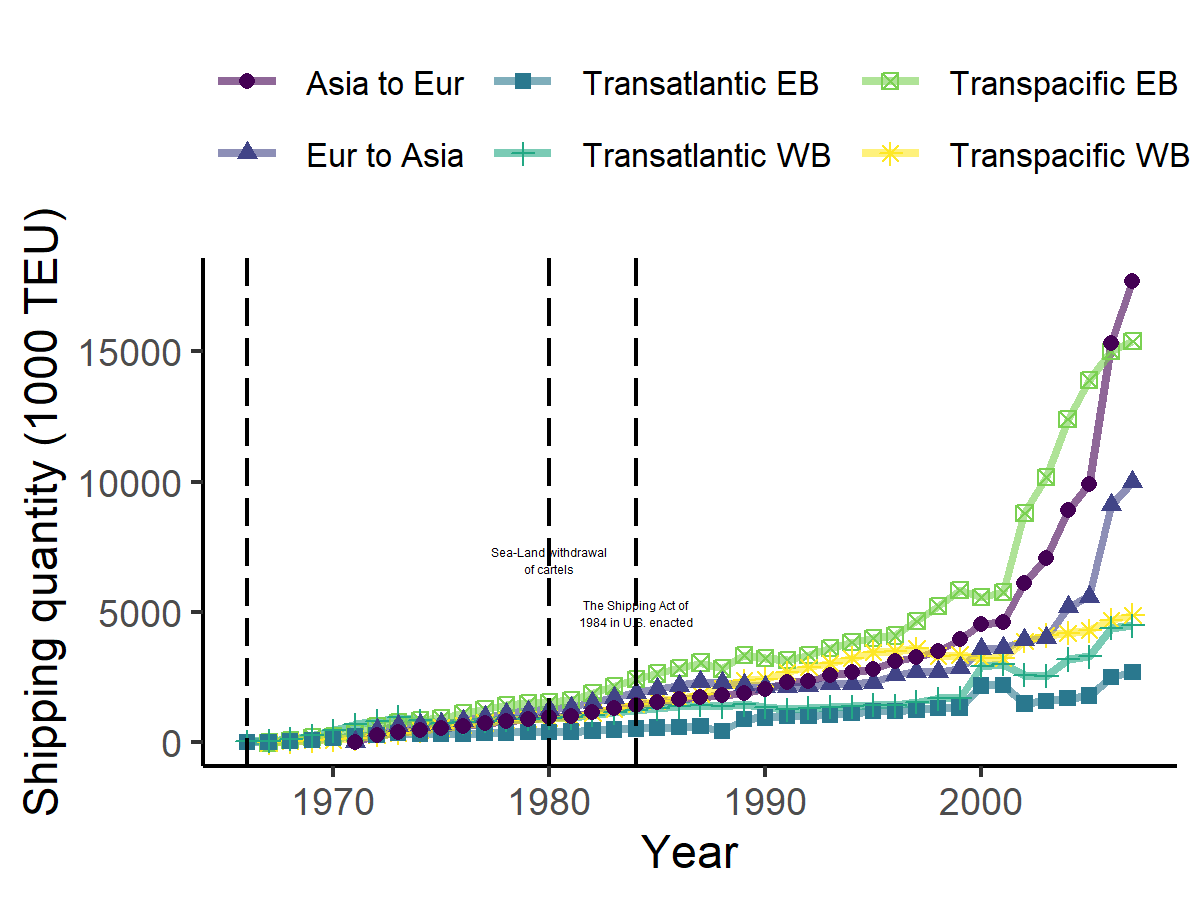
\includegraphics[height = 0.5\textheight]{figuretable/container_shipping_quantity_each_route.png}

\end{center}
\caption{The trend of the container shipping quantity. The trend before 1976 is based on ship-level carrying capacity information in each route.}
\label{fg:container_shipping_quantity_each_route}
\end{figure}


\subsection{Newbuilding, Secondhand, and Scrap prices}
We provide a recommendation for constructing newbuilding, secondhand, and scrap prices for container ships from 1967. Our data were collected from a series of \textit{Review (1971-1998)} published by Fearnley and \textit{Lloyd's Shipping Economist (1983-1990)} published by Lloyd's of London Press. 

\subsubsection{Newbuilding prices}
We collected industry-year-level newbuilding prices per 18000 DWT bulk ships from \textit{Review (1971-1998)}. ). Using the overlapped year, we converted the prices into consistent prices under the assumption that the conversion rate is invariant across years. Then, we divided the price per 12000 dwt by 10 to convert to the price per 1200 TEU and then converted it into the price per TEU. Finally, we converted bulk prices into container prices based on \textit{Lloyd's Shipping Economist (1983-1990)}.

\subsubsection{Secondhand prices}
We collected industry-year-level secondhand prices per 16000 DWT CSD (liner type) ships from \textit{Review (1971-1998)}. Using the overlapped year, we converted the prices into consistent prices under the assumption that the conversion rate is invariant across years.

We assume a fixed depreciation rate ($= X$) and fixed conversion rate ($= a$) for 1981 and 1983, and observe the following:
\begin{align*}
    1981: 2.7 + 2X &= 16.0a \quad\text{(18-year depreciation)}\\
    1983: 0.8 + 0X &=11a \quad\text{(20-year depreciation)}
\end{align*}
We solve the system of equation for $X$ and $a$. To obtain the price per $1600dwt+15X$, we multiplied the above price by 12000/16000 and obtained the price per 12000dwt. Then, we divided the price by 10 to convert it to the price per 1200TEU. We then converted it into the price per TEU of 5 years ship by dividing it by 1200. Finally, we converted the liner prices into container prices based on \textit{Lloyd's Shipping Economist (1983-1990)}.


\subsubsection{Scrap prices}

We collected industry-year-level scrap prices per LTD in the Far-East. Using the overlapped year, we converted the prices into consistent prices under the assumption that the conversion rate is invariant across years. We then divided per LTD by four to obtain the price per dwt, multiply it by 10, and convert it into the price per TEU.\footnote{The rate is based on \textit{https://nippon.zaidan.info/seikabutsu/2002/00264/contents/030.htm}.}

